\subsection{Universidad París Descartes - Francia}
Presentamos en la siguiente tabla los resultados obtenidos del último monitoreo.

\bigskip

\begin{tabular}{ | l | c | c | c | c |}
 \hline                 
   Hop & IP &  RTT promedio (s)  & deltaRTT promedio & Ubicación\\
 \hline 
   1 & 192.168.0.1 & 0,006502 & 0,006502 & Argentina - Buenos Aires\\ 
 \hline 
   2 & 200.89.164.189 & 0,025426 & 0,018924 & Argentina - Buenos Aires\\ 
  \hline 
   3 & 200.89.165.5 & 0,022739 & 0 & Argentina - Buenos Aires\\ 
  \hline 
   4 & 200.89.165.250 & 0,023967 & 0,001227 & Argentina - Buenos Aires\\ 
  \hline 
   5 & 206.165.31.213 & 0,023886 & 0 & Estados Unidos\\ 
  \hline 
   6 & 67.16.139.18 & 0.153896 & 0,130009 & Estados Unidos - Manhattan\\ 
  \hline 
   7 & 213.248.76.189 & 0,147402 & 0 & Europa (Telia Network Services)\\ 
  \hline 
   8 & 62.115.143.64 & 0,173705 & 0,026303 & Europa (Telia Network Services UK)\\ 
  \hline 
   9 & 213.155.130.86 & 0,174316 & 0,000610 & Europa (Telia Network Services UK)\\ 
  \hline 
   10 & 80.239.132.130 & 0,183801 & 0,009485 & Alemania (Telia AB/Telia Int. Carrier)\\ 
  \hline 
   11 & 195.2.30.46 & 0,249497 & 0,065696 & Europa\\ 
  \hline 
   12 & 195.2.28.154 & 0,244204 & 0 & Europa\\ 
  \hline 
   13 & 195.2.10.145 & 0,243621 & 0 & Europa\\ 
  \hline 
   14 & 195.10.54.66 & 0,269441 & 0,025820 & Francia (Dyson Ltd)\\ 
  \hline 
   15 & 193.51.177.25 & 0,271685 & 0,002243 & Francia - Paris\\ 
  \hline 
   16 & 193.51.177.116 & 0,258662 & 0 & Francia - Paris\\ 
  \hline 
   17 & 193.51.181.101 & 0,258660 & 0 & Francia - Paris\\
  \hline 
   18 & 195.221.127.166 & 0,269296 & 0,010635 & Francia - Paris\\
  \hline 
   19 & 193.51.86.16 & 0,256802 & 0 & Francia\\
  \hline 
   20 & 193.51.181.101 & 0,258082 & 0,001279 & Francia\\
  \hline 
   21 & 193.51.181.101 & 0,254919 & 0 & Francia\\
  \hline 
   22 & 193.51.181.101 & 0,255926 & 0,001007 & Francia\\
  \hline 
   23 & 193.51.181.101 & 0,254769 & 0 & Francia\\
  \hline 
   24 & 193.51.181.101 & 0,256566 & 0,001797 & Francia\\    
 \hline 
\end{tabular}

\bigskip

Con estos datos hemos obtenido que los $\Delta$ $RTT$ siguen una distribución normal con una probabilidad del 99,5$\%$ ($\alpha$ $=$ 0,005).
Se ha realizado el test de $Grubbs$ y nos ha devuelto que los $outliers$ se encuentran en los saltos 6 y 11.\\

A continuación mostramos que ocurre con los $RTT$ promedio de cada salto y con los $zScore$ promedio de cada salto:

\begin{figure}[H]
\centering
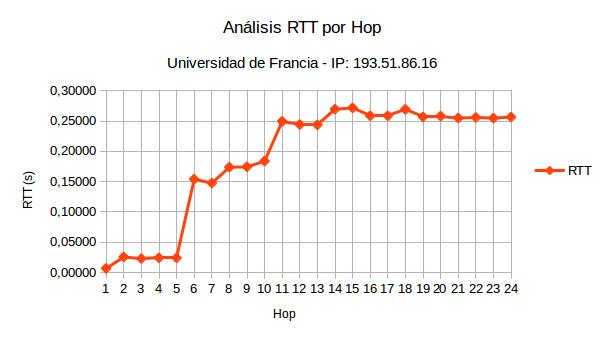
\includegraphics[width=1\textwidth]{graficos/rTT_Francia.jpg}
\caption{RTT promedio por hop - Universidad de Francia}
\label{francia_rtt}
\end{figure}

\begin{figure}[H]
\centering
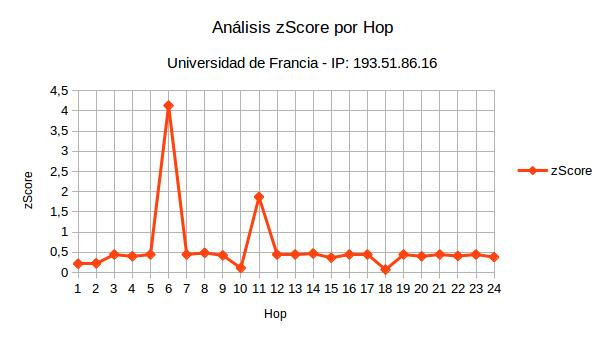
\includegraphics[width=1\textwidth]{graficos/zScore_Francia.jpg}
\caption{zScore promedio por hop - Universidad de Francia}
\label{francia_zs}
\end{figure}

En ambos gráficos se puede apreciar como en los saltos 6 y 11 (los que nos habían dado como $outliers$ en el test de $Grubbs$) hay un cambio abrupto 
en la distribución de los datos. En el gráfico de $RTT$ podemos notar cómo sube de golpe el $RTT$ promedio. En el otro gráfico podremos observar cómo 
se forman picos en estos saltos.\\

Nos ha llamado la atención que figuren dos $outliers$ cuando el enlace submarino debería ser solamente uno para ir hacia Francia. 
Verificando las ubicaciones de los host intermedios notamos que el primer $outlier$ corresponde a un host que se encuentra en Estados Unidos 
(el cual nosotros desde Argentina estamos a más de 8000 kilómetros). El salto 5, según nos indica la herramienta de geolocalización, se encontraría
en Estados Unidos pero no creemos que sea cierto dado que el $RTT$ es muy similar a los hosts ubicados en Argentina.\\

El segundo $outlier$ detectado corresponde al salto 11 donde ya nos ubicamos en un host europeo. Aquí claramente ya hemos atravesado un 
enlace submarino desde Estados Unidos hacia Europa. También nos ha llamado la atención al localizar los hosts anteriores del salto 11: los hemos 
localizado en Europa. Sin embargo no tienen un cambio de $RTT$ significativo por lo que estimamos que se encuentran en Estados Unidos. Los saltos 7, 8, 9 y 10
corresponden a hosts de la empresa de telecomunicaciones Telia y estimamos que debe contratar servicios en Estados Unidos. Por este motivo no notamos 
en los $RTT$ cambios abruptos ni picos en los $zScore$ obtenidos.\\

Para los demás saltos hemos notado que los $\Delta$ $RTT$ son similares y los host debe estar equidistantes hasta llegar al host destino dado que no 
hemos observado valores atípicos.\\

A continuación hemos trazado en un mapa la ruta de nuestro host hasta el host destino ubicado en Francia:
\begin{figure}[H]
\centering
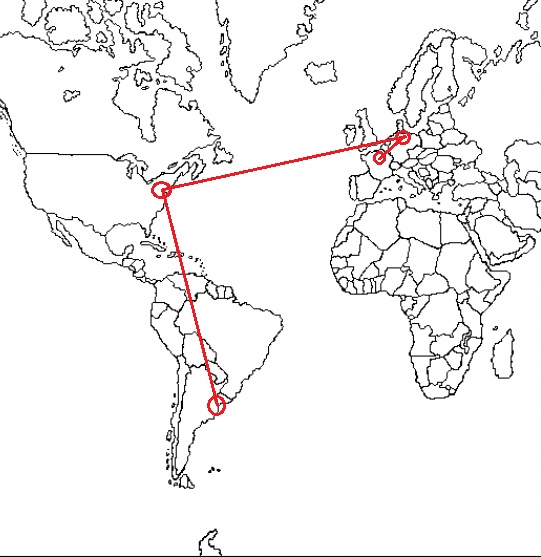
\includegraphics[width=0.8\textwidth]{graficos/mapa_francia.jpg}
\caption{Ruta en Internet - Universidad de Francia}
\label{francia_zs}
\end{figure}

